\subsection{Three-Dimensional Model}

\frame{
   \frametitle{3D Model -- Basics}
   \begin{columns}
      \column{.75\textwidth}
%	 \vspace{-.5cm}
	 \begin{itemize}
	    \item Structural Representation -- 2D
	    \item Vertical dimension is time -- 1D 
	       \begin{itemize}
	       \item Objects' Behavior Evolution
	       \item States and Links
	       \end{itemize}
	       \vspace{.5cm}
	    \item Interaction Techniques
%	       \begin{itemize}
%		  \item Notion of a Camera
%		  \item Rotation
%		  \item Translation
%		  \item Objects Animation
%		  \item Replay step-by-step
%	       \end{itemize}
	    \end{itemize}
      \column{.30\textwidth}
%	 \vspace{-.5cm}
	 \begin{figure}[!htb]
	 \centerline{
	    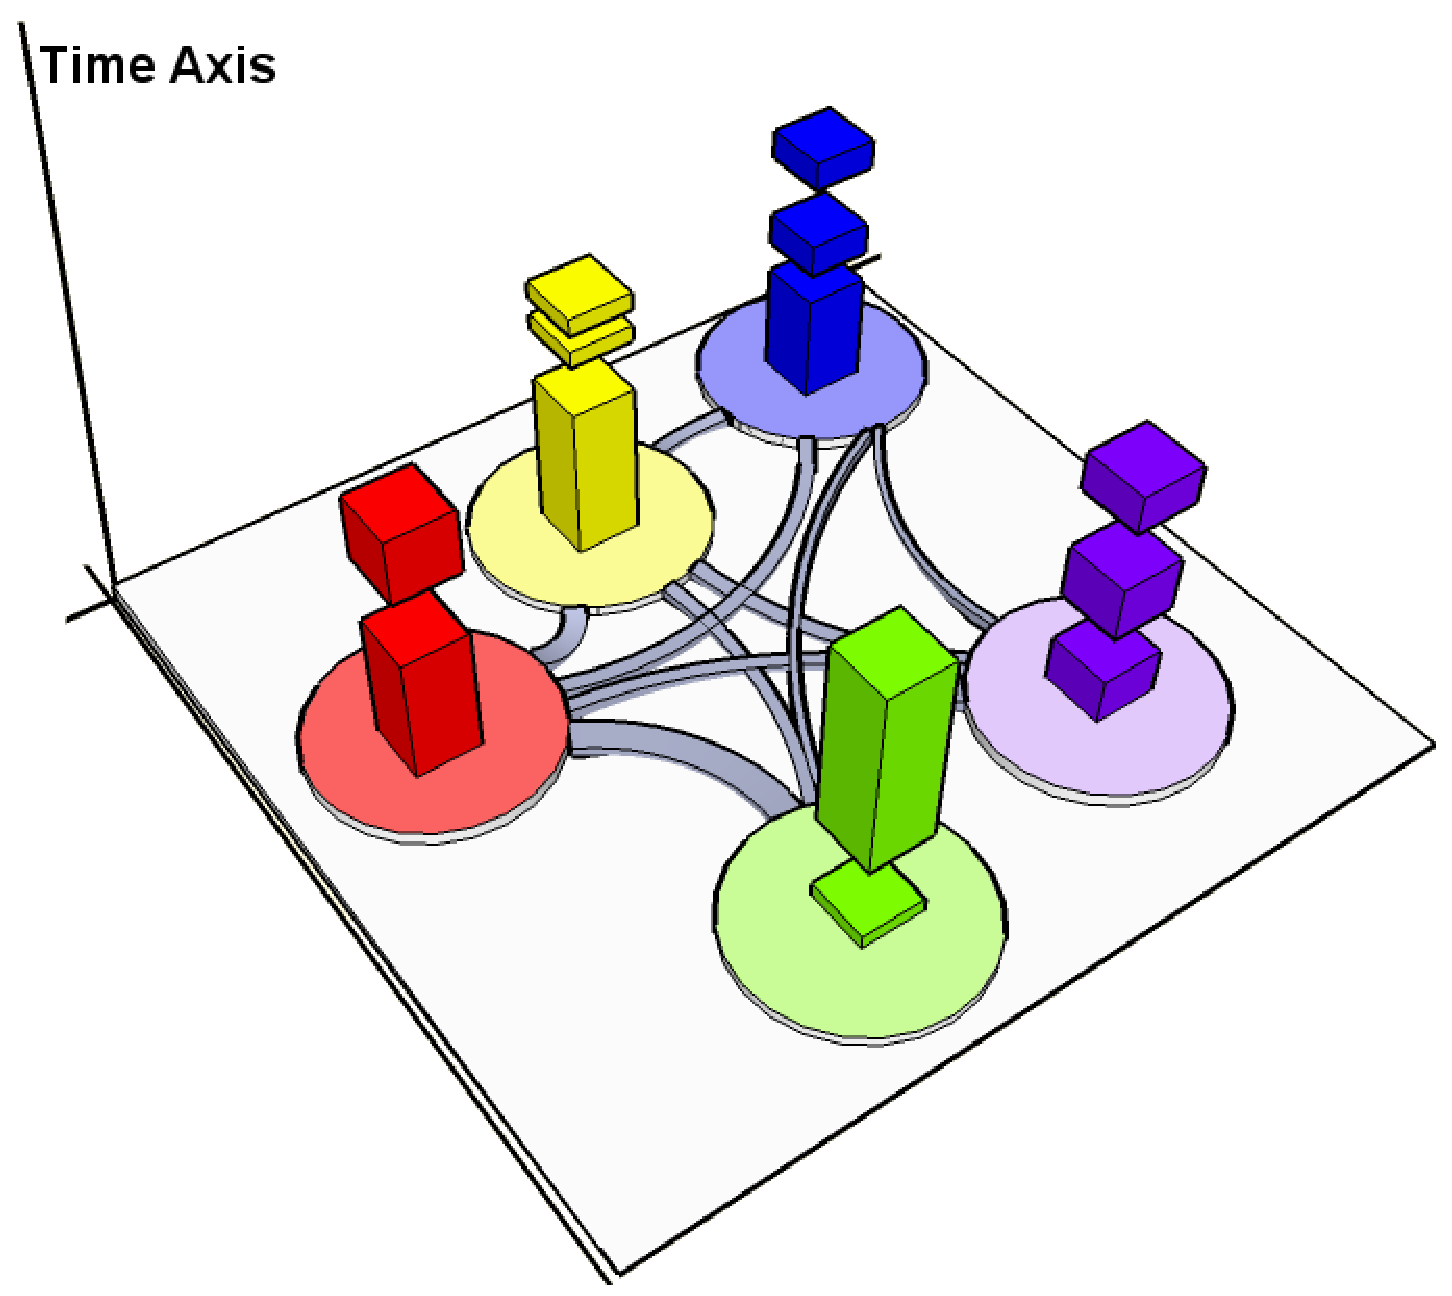
\includegraphics[width=1.2\textwidth]{img/5proc-basic-start.pdf}}
%	 \centerline{
%	    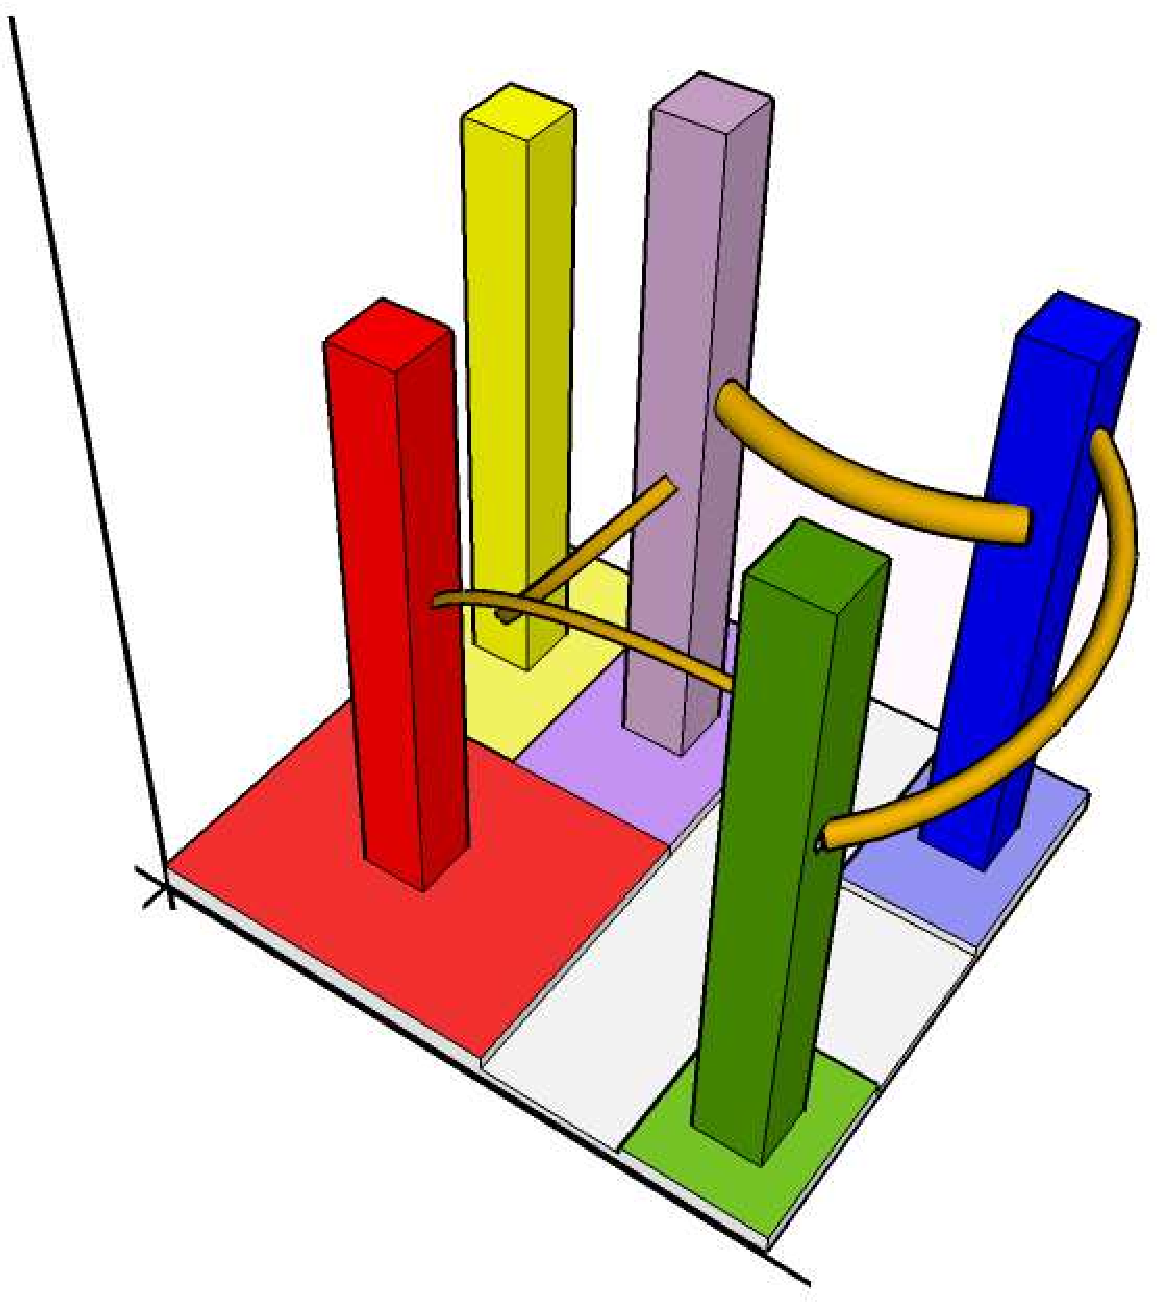
\includegraphics[width=1.2\textwidth]{img/5proc-treemap-com.pdf}}
	 \end{figure}
   \end{columns}
}

%\frame{
%   \frametitle{3D Model - Differences from existing tools}
%   \begin{itemize}
%      \item 3D Statistical Representation
%	 \begin{itemize}
%	 \item Pablo $\rightarrow$ 3D Scatter Plot
%	 \item Paradyn $\rightarrow$ 3D Terrain
%	 \item ParaProf $\rightarrow$ Triang Mesh, 3D Bar and 3D Scatter Plot
%	 \end{itemize}
%      \item 3D Behavioral Representation
%	 \begin{itemize}
%	 \item ParaProf $\rightarrow$ 2 metrics and time
%	 \item Virtue $\rightarrow$ the time-tunnel view
%	 \end{itemize}
%      \vspace{.5cm}
%      %\item Lack of structural representation
%   \end{itemize}
%
%   \vfill
%
%   \begin{block}{Our Approach}
%   \begin{itemize}
%   \item Presence of a timeline to show objects' evolution
%   \item Multiple Configurations in the visualization base
%   \end{itemize}
%   \end{block}
%}

\frame{
   \frametitle{3D Model - Visualization}
   \begin{itemize}
   \item<1-> How objects are represented in 3D
   \item<2-> Rendering the Network Topology + Comm. Pattern
   \end{itemize}

   \vfill

   \begin{minipage}{\textwidth}
   \centering
   \includegraphics<1>[width=\textwidth]{img/3d-states-link.pdf}
%   \includegraphics<2>[width=\textwidth]{img/3d-base-case1.pdf}
   \includegraphics<2>[width=\textwidth]{img/3d-base-case2.pdf}
%   \includegraphics<4>[width=\textwidth]{img/3d-base-case3.pdf}
   \end{minipage}
}
